\subsection{Underflow}
    Arithmetic underflow is a condition that can happen in computers, underflow is caused when a number is smaller than the minimum non-negative number a computer can store, and will therefore cause rounding errors bigger than usual. This can be seen by looking at how a computer stores numbers in binary, by looking at a 2 byte binary number with one byte before the decimal point and one byte after we get:\\

\begin{table}[!h]
    \begin{tabular}{|l|l|l|}
        \hline
        Bit number & Value    & Decimal \\ \hline
        3          & $2^3$    & 8       \\ 
        2          & $2^2$    & 4       \\ 
        1          & $2^1$    & 2       \\ 
        0          & $2^0$    & 1       \\ 
        -1         & $2^{-1}$ & 0.500   \\ 
        -2         & $2^{-2}$ & 0.250   \\ 
        -3         & $2^{-3}$ & 0.125   \\ 
        -4         & $2^{-4}$ & 0.0625  \\
        \hline
    \end{tabular}
\end{table}

	\begin{figure}
		\centering
		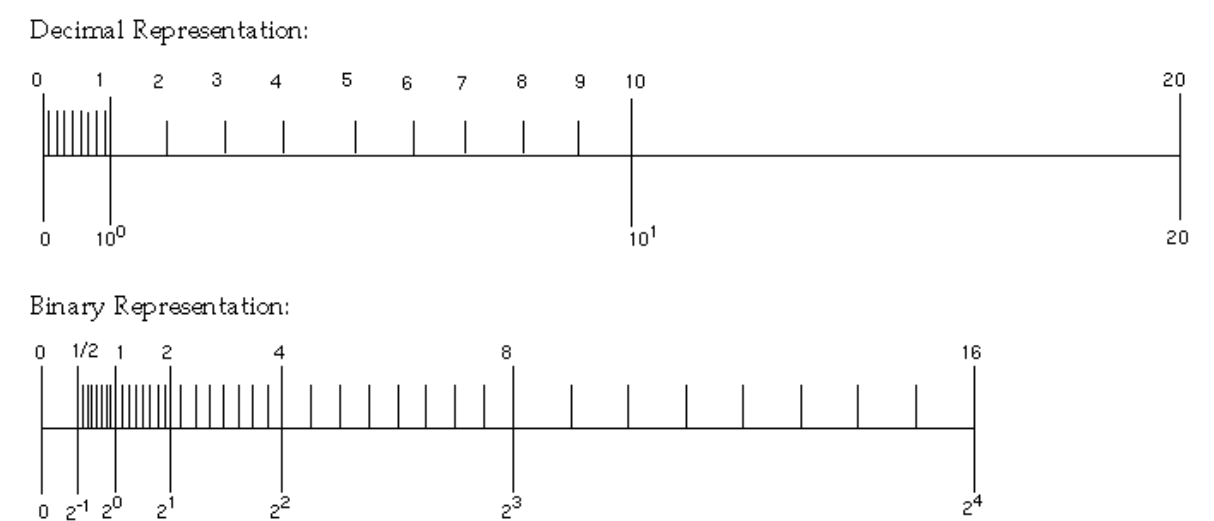
\includegraphics[width=1\linewidth]{pictures/binary_underflow.png}
		\caption{Binary representation}
		\label{fig:binary_underflow}
	\end{figure}


    This makes the smallest number $0.0625$, any value less than this will get rounded either down to zero or up to $0.0625$. The smallest number in binary is:

    $$0000.0001 = 0.0625$$

\subsubsection{Does it matter}
In many cases underflow could be neglected, if the program is not working with very small numbers, or the accuracy is not that important, but in some cases and for solid programs the program should be able to detect underflow. If an algorithm is working with probabilities and a very small number is inaccurate or zero, computing calculations with this number could cause big problems, especially in cases where the program will try to divide with zero. This is a very important event to be concerned of when working with probabilities that gets very small.  

\subsubsection{How to work around it}
In this project there is a high probability that very small numbers will occur, this demands a work around to the underflow problem. One possible work around is called \textit{log odds} this method maps values $[0;1]$ to $[-\infty; \infty]$. The log odds for state \textit{A} is the logarithm of the probability for state $A$ divided by the probability for state $\neg A$.\\

    $$\frac{p(A)}{p(\neg A)} = \frac{p(A)}{1-p(A)}$$

    $$l(A) = \log \frac{p(A)}{1-p(A)}$$

    The mapping is shown on the graph below:\\
	\begin{figure}
		\centering
		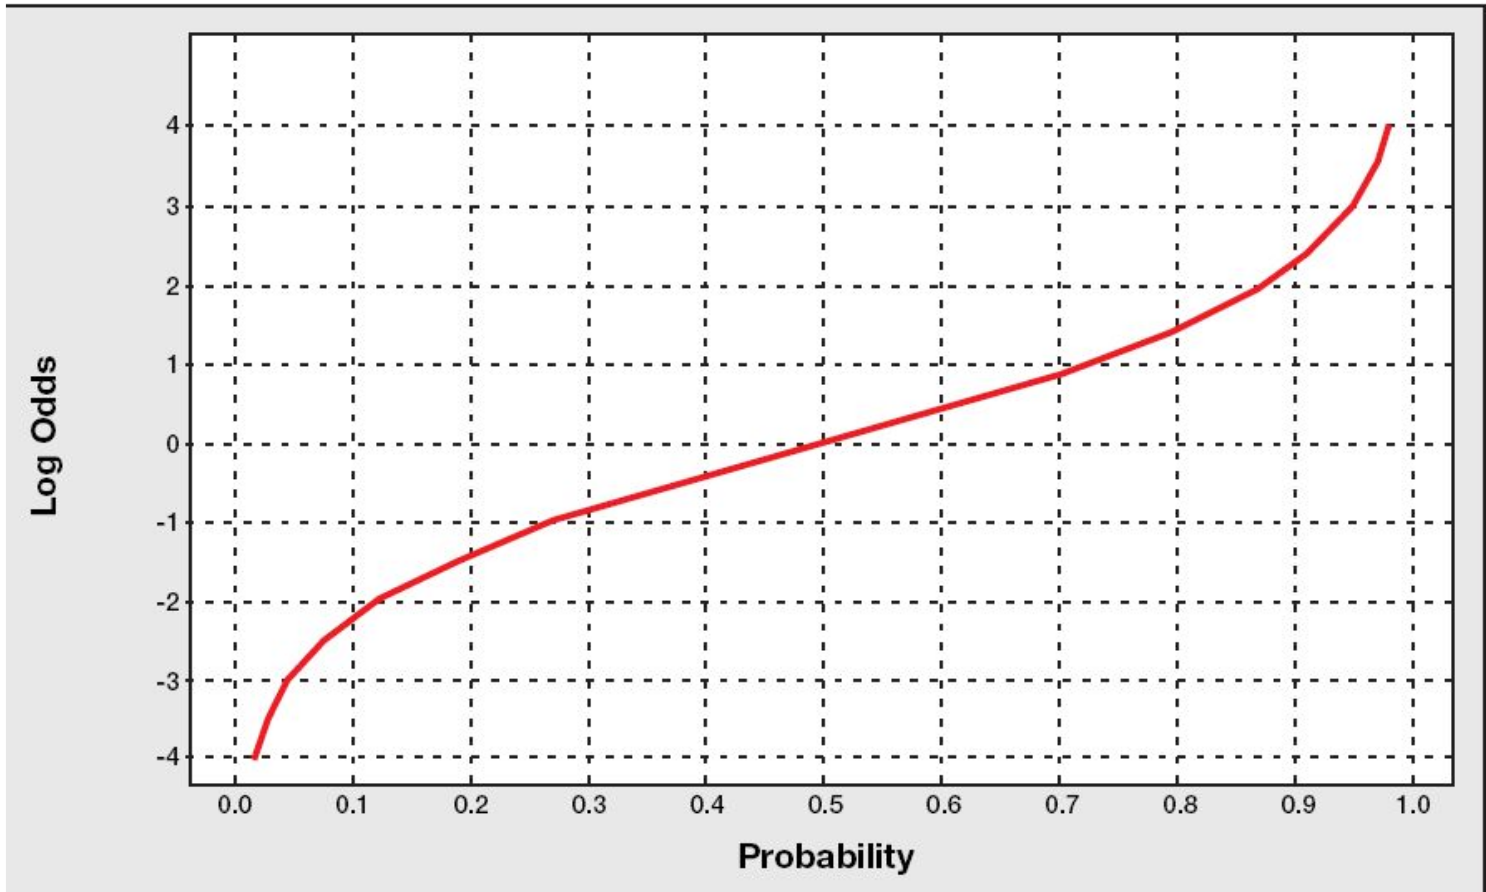
\includegraphics[width=1\linewidth]{pictures/logodds_mapping.png}
		\caption{Mapping for log odds}
		\label{fig:log_odds}
	\end{figure}

    Another way to work around the problem is with Pythons \textit{decimal} library, this library makes it possible to store decimal numbers with exact precision and detect underflow. It possible to define how many decimals you want on numbers in the decimal library.

To determine what method works best, some tests needs to be done, in order to figure out when the \textit{log odds} would be prefer over the \textit{decimal} library.
